\documentclass[12pt]{article}
\usepackage{graphicx,import}
\usepackage[svgnames]{xcolor} 
\usepackage{fancyhdr}
\usepackage{subfig}
\usepackage{hyperref}
\usepackage{enumitem}
\usepackage{cite}
\usepackage[many]{tcolorbox}
\usepackage{listings }
\usepackage[a4paper, total={6in, 8in} , bottom = 25mm , top = 25mm, headheight = 1.25cm , includehead,includefoot,heightrounded ]{geometry}
\usepackage{afterpage}
\usepackage{amssymb}
\usepackage{pdflscape}
\usepackage{gensymb}
\usepackage{textcomp}
\usepackage{tikz,pgfplots}
\usepackage{xecolor}
\usepackage{rotating}
\usepackage{pdfpages}
\usepackage{fancyvrb}
\usepackage[Kashida]{xepersian}
\usepackage[T1]{fontenc}
\usepackage{tikz}
\usepackage[utf8]{inputenc}
\usepackage{PTSerif} 
\usepackage{seqsplit}

\usepackage[edges]{forest}

\usepackage{listings}
\usepackage{xcolor}

\hypersetup{
	colorlinks   = true, %Colours links instead of ugly boxes
	urlcolor     = blue, %Colour for external hyperlinks
	linkcolor    = blue, %Colour of internal links
	citecolor   = red %Colour of citations
}

\definecolor{codegreen}{rgb}{0,0.6,0}
\definecolor{codegray}{rgb}{0.5,0.5,0.5}
\definecolor{codepurple}{rgb}{0.58,0,0.82}
\definecolor{backcolour}{rgb}{0.95,0.95,0.92}

\NewDocumentCommand{\codeword}{v}{
	\texttt{\textcolor{blue}{#1}}
}
\lstset{language=java,keywordstyle={\bfseries \color{blue}}}

\lstdefinestyle{mystyle}{
	backgroundcolor=\color{backcolour},   
	commentstyle=\color{codegreen},
	keywordstyle=\color{magenta},
	numberstyle=\tiny\color{codegray},
	stringstyle=\color{codepurple},
	basicstyle=\ttfamily\normalsize,
	breakatwhitespace=false,         
	breaklines=true,                 
	captionpos=b,                    
	keepspaces=true,                 
	numbers=left,                    
	numbersep=5pt,                  
	showspaces=false,                
	showstringspaces=false,
	showtabs=false,                  
	tabsize=2
}

\lstset{style=mystyle}

\settextfont[Scale=1.2 ,BoldFont={Bahij Nazanin-Bold.ttf} , ItalicFont = {IRNazaninIranic.ttf}]{Bahij Nazanin-Regular.ttf}
\setlatintextfont[Scale = 1.0]{Garamond}
\DefaultMathsDigits 
\DeclareMathSizes{11}{19}{13}{9} 
%\DeclareMathSizes{12}{14.4}{8}{9}





\newenvironment{changemargin}[2]{%
	\begin{list}{}{%
			\setlength{\topsep}{0pt}%
			\setlength{\leftmargin}{#1}%
			\setlength{\rightmargin}{#2}%
			\setlength{\listparindent}{\parindent}%
			\setlength{\itemindent}{\parindent}%
			\setlength{\parsep}{\parskip}%
		}%
		\item[]}{\end{list}}


\definecolor{foldercolor}{RGB}{124,166,198}

\tikzset{pics/folder/.style={code={%
			\node[inner sep=0pt, minimum size=#1](-foldericon){};
			\node[folder style, inner sep=0pt, minimum width=0.3*#1, minimum height=0.6*#1, above right, xshift=0.05*#1] at (-foldericon.west){};
			\node[folder style, inner sep=0pt, minimum size=#1] at (-foldericon.center){};}
	},
	pics/folder/.default={20pt},
	folder style/.style={draw=foldercolor!80!black,top color=foldercolor!40,bottom color=foldercolor}
}

\forestset{is file/.style={edge path'/.expanded={%
			([xshift=\forestregister{folder indent}]!u.parent anchor) |- (.child anchor)},
		inner sep=1pt},
	this folder size/.style={edge path'/.expanded={%
			([xshift=\forestregister{folder indent}]!u.parent anchor) |- (.child anchor) pic[solid]{folder=#1}}, inner xsep=0.6*#1},
	folder tree indent/.style={before computing xy={l=#1}},
	folder icons/.style={folder, this folder size=#1, folder tree indent=3*#1},
	folder icons/.default={12pt},
}

\begin{document}
	
	
	%%% title pages
	\begin{titlepage}
		\begin{center}
			
			\vspace*{0.7cm}
			
			
\includegraphics[width=0.4\textwidth]{sharif1.png}\\
			\vspace{0.5cm}
			\textbf{ \Huge{\emph  ﺷﺒﻜﻪ‌های کامپیوتری} }\\
			\vspace{0.5cm}
			\textbf{ \Large{ تمرین دوم} }
			\vspace{0.2cm}
			
			
			\large \textbf{دانشکده مهندسی کامپیوتر}\\\vspace{0.2cm}
			\large   دانشگاه صنعتی شریف\\\vspace{0.2cm}
			\large   ﻧﯿﻢ سال دوم 00-99 \\\vspace{0.2cm}
			\noindent\rule[1ex]{\linewidth}{1pt}
			استاد:\\
			\textbf{{جناب آقای دکتر جعفری}}
			
			
			\vspace{0.15cm}
			نام و نام خانوادگی:\\
			
			
			\textbf{{امیرمهدی نامجو - 97107212}}
		\end{center}
	\end{titlepage}
	%%% title pages
	
	
	%%% header of pages
	\newpage
	\pagestyle{fancy}
	\fancyhf{}
	\fancyfoot{}
	\cfoot{\thepage}
	\chead{تمرین دوم}
	\rhead{
\includegraphics[width=0.1\textwidth]{sharif.png}}
	\lhead{امیرمهدی نامجو}
	%%% header of pages
	
	\KashidaOff
	
	\section{سوال اول}
	
	\textbf{توجه: امکان زوم بر روی تمامی تصاویری که در متن قرار دارند وجود دارد.}
	
	\begin{enumerate}
		
		\item
		
		وضعیت درخواست‌های DNS رد و بدل شده برای فیسبوک به صورت زیر است:
		
		\begin{center}
			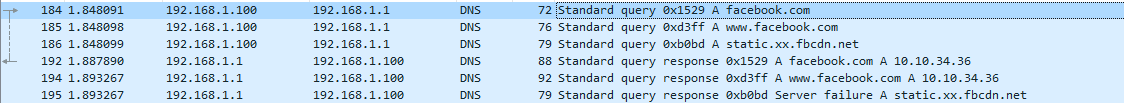
\includegraphics[width = 1.0 \textwidth]{images/1.png}
		\end{center}

سه درخواست اول از کامپیوتر من به روتر رفته‌اند و سه مورد بعدی جواب‌هایی هستند که از روتر به کامپیوتر من برگشته اند. مشاهده می‌کنیم آدرس آی‌پی که برای فیسبوک برگشته است
\lr{\Verb+10.10.34.36+}
است.

این آدرس آی‌پی جزو دسته آی‌پی‌های رزرو شده است که بین
\lr{\Verb+10.0.0.0+}
تا
\lr{\Verb+10.255.255.255+}
قرار دارد. این آدرس آی‌پی‌ها مربوط به شبکه‌های خصوصی هستند و عملا به سایت خاصی در اینترنت نگاشت نشده‌اند. این یعنی \lr{DNS} سرور، آدرسی را برای سایت \lr{Facebook} برگردانده که عملا مربوط به شبکه عمومی اینترنت نمی‌شود و یک آدرس در شبکه خصوصی است که عملا در کامپیوتر من وجود  نداشته و نتیجتا کروم با خطای
\lr {\Verb+This site can’t be reached+}
و
\lr{\Verb+ERR\_CONNECTION\_TIMED\_OUT+}
متوقف می‌شود.
	
	با بررسی تنظیمات مودم متوجه شدم که DNS-Server پیش‌فرض آن به صورت \lr{\Verb+46.224.1.220+} است که با \lr{IpLookup} کردن آن، متوجه می‌شویم که این آی‌پی متعلق به \lr{\Verb+ns5.hiweb.ir+} یعنی Nameserver «های‌وب» در ایران است و منطقی است که فیلترینگ روی این Nameserver داخلی اعمال شده باشد و در نتیجه DNS به آن نتیجه نامعتبری برای \lr{facebook.com} که یک سایت فیلتر شده است برگرداند.
	
	
	\item
	
	وضعیت درخواست DNS برای سایت اوراکل به صورت زیر است:
	
		\begin{center}
		
\includegraphics[width = 1.0 \textwidth]{images/2.png}
	\end{center}
	
	


وضعیت خروجی برگدانده شده برای آن به صورت زیر است:

\begin{latin}
	\begin{verbatim}
		Answers
		www.oracle.com: type CNAME, class IN,
		 cname ds-www.oracle.com.edgekey.net
		Name: www.oracle.com
		Type: CNAME (Canonical NAME for an alias) (5)
		Class: IN (0x0001)
		Time to live: 497 (8 minutes, 17 seconds)
		Data length: 31
		CNAME: ds-www.oracle.com.edgekey.net
		ds-www.oracle.com.edgekey.net: type CNAME, class IN,
		 cname e2581.dscx.akamaiedge.net
		Name: ds-www.oracle.com.edgekey.net
		Type: CNAME (Canonical NAME for an alias) (5)
		Class: IN (0x0001)
		Time to live: 451 (7 minutes, 31 seconds)
		Data length: 24
		CNAME: e2581.dscx.akamaiedge.net
		e2581.dscx.akamaiedge.net: type A, class IN, addr 23.14.117.40
		Name: e2581.dscx.akamaiedge.net
		Type: A (Host Address) (1)
		Class: IN (0x0001)
		Time to live: 497 (8 minutes, 17 seconds)
		Data length: 4
		Address: 23.14.117.40
		
	\end{verbatim}
\end{latin}
	
	جواب اول مشخص می‌کند که \lr{\Verb+www.oracle.com+} در اصل یک \lr{Alias} برای یک آدرس دیگر است.
	
	 جواب دوم مشخص می‌کند که آدرس مشخص شده بعدی یعنی
	 
	  \lr{\Verb+ds-www.oracle.com.edgekey.net+}
	  
	   هم یک \lr{Alias} برای آدرس دیگری است. آدرس نهایی یعنی \lr{\Verb+e2581.dscx.akamaiedge.net+} به یک آدرس آی‌پی واقعی مپ شده است. این آدرس ای‌پی یعنی \lr{\Verb+23.14.117.40+} مربوط به یکی از \lr{CDN} های شرکت \lr{Akamai} است. این \lr{CDN} در ترکیه واقع شده است و براساس موقعیت مکانی من که ایران بوده، نزدیک‌ترین \lr{CDN} تشخیص داده شده مربوط به کشور ترکیه بوده است. با این وجود در نهایت شاهد این هستیم که سایت \lr{Oracle} باز نمی‌شود و با خطاهای 
	\lr {\Verb+This site can’t be reached+}
	و
	\lr{\Verb+ERR\_CONNECTION\_TIMED\_OUT+}
	مواجه می‌شویم. این خطاها این بار به خاطر فیلترینگ نیستند بلکه به خاطر تحریم است.
	
	
		
	
	
	\item
	
	پیش از بررس نتایج باید بررسی کنیم که آی‌پی آدرس DNS-Server های شکن متعلق به کجاست. در سایت دو آی‌پی آدرس قرار گرفته است. اولین مورد \lr{\Verb+178.22.122.100+} است که متعلق به شرکت آسیاتک (\lr{Asiatech Data Transmission company}) بوده و دومین آی‌پی \lr{\Verb+185.51.200.2+} است که متعلق به شرکت مهندسی صفرویک پرداز (\lr{Sefroyek Pardaz Engineering Co. LTD}) است.
	
با انجام تنظیمات مربوطه و وارد کردن آدرس Oracle داریم:

			\begin{center}
		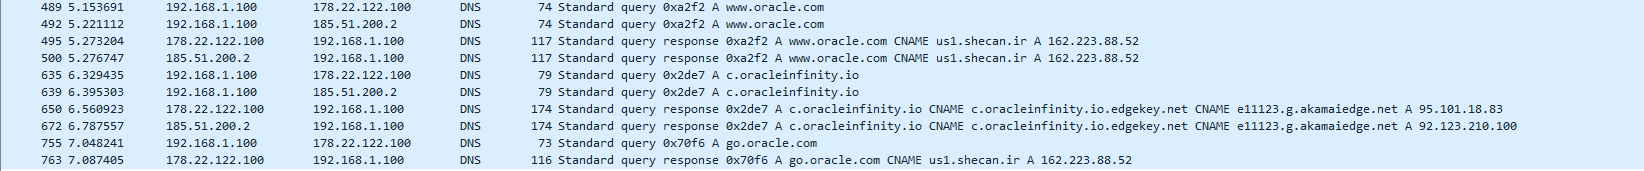
\includegraphics[width = 1.0 \textwidth]{images/3.png}
	\end{center}
	
	همان طور که در تصویر مشخص است در نتیجه درخواست آدرس \lr{\Verb+www.oracle.com+} خروجی به این صورت بوده که این آدرس Alias ای برای آدرس \lr{\Verb+us1.shecan.ir+} است و آدرس آی‌پی \lr{\Verb+162.223.88.52+} گزارش شده است. این آدرس آی‌پی در آمریکا قرار داشته و متعلق به شرکتی به اسم ColoUp است. با مراجعه به سایت این شرکت می‌توان مشاهده کرد که این شرکت مرتبط به خدمات شبکه است و البته بخش گزارش خطا به زبان فارسی هم دارد در نتیجه می‌توان به این نتیجه رسید که با شکن در ارتباط است.
			\begin{center}
		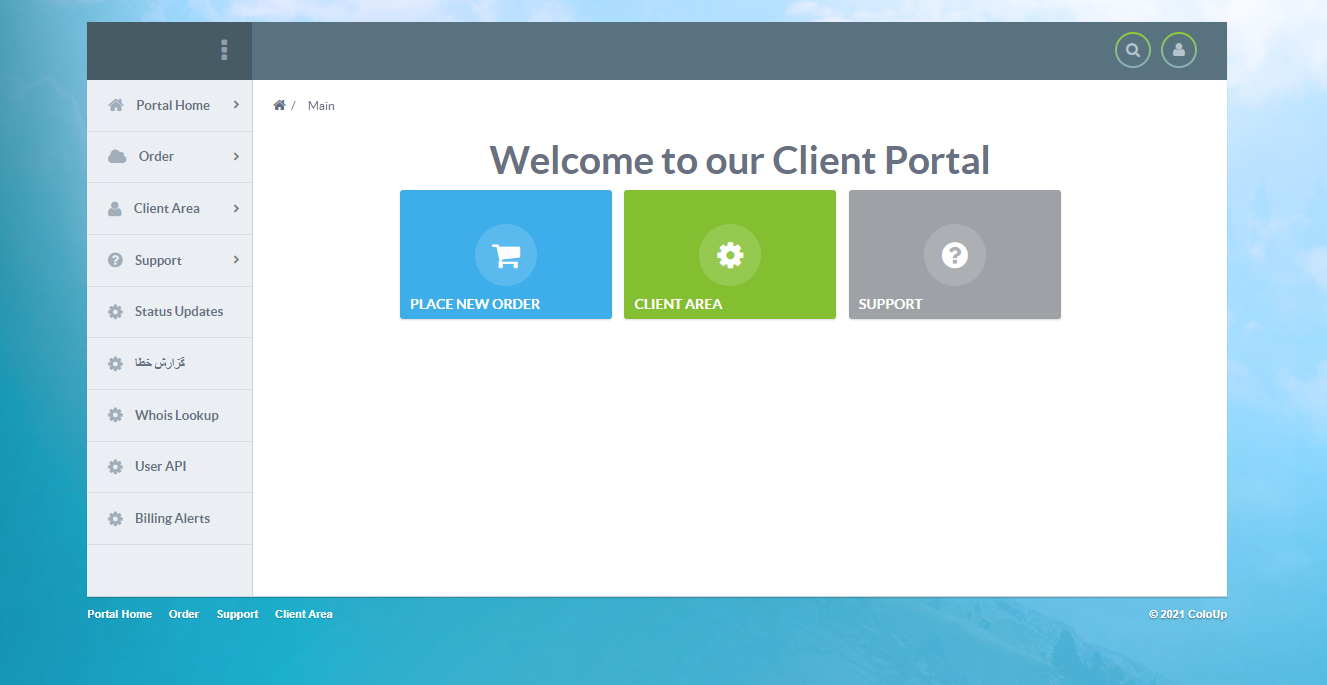
\includegraphics[width = 0.5 \textwidth]{images/4.png}
	\end{center}

خروجی برگردانده شده به صورت زیر است:

\begin{latin}
	\begin{verbatim}
		Answers
		www.oracle.com: type CNAME, class IN, cname us1.shecan.ir
		Name: www.oracle.com
		Type: CNAME (Canonical NAME for an alias) (5)
		Class: IN (0x0001)
		Time to live: 118 (1 minute, 58 seconds)
		Data length: 15
		CNAME: us1.shecan.ir
		us1.shecan.ir: type A, class IN, addr 162.223.88.52
		Name: us1.shecan.ir
		Type: A (Host Address) (1)
		Class: IN (0x0001)
		Time to live: 214 (3 minutes, 34 seconds)
		Data length: 4
		Address: 162.223.88.52
		
	\end{verbatim}
	\end{latin}

سایر موارد مربوط به \lr{Oracle} که مشاهده می‌شود، مربوط به \lr{CDN} ها و موارد متفرقه دیگری هستند که تحریم نبوده و همان \lr{IP} اصلی آن ها برگردانده شده است. البته \lr{\Verb+go.oracle.com+} هم تحریم است و برای آن هم آدرس مربوط به \lr{\Verb+ us1.shecan.ir+} برگردانده شده است.

بدین ترتیب به نظر می‌رسد که درخواست‌هایی که ما برای سایت \lr{Oracle} می‌فرستیم به جای این که مستقیما به سایت \lr{Oracle} برود، به سایت واسطه‌ای که آدرس آن \lr{\Verb+ us1.shecan.ir +} است می‌رود و سپس از طریق این سایت به \lr{Oracle} منتقل شده و جواب‌ها هم از طریق همین سایت با آی‌پی 
\lr{\Verb+ 162.223.88.52 +}
برای ما بر می‌گردد:
		\begin{center}
	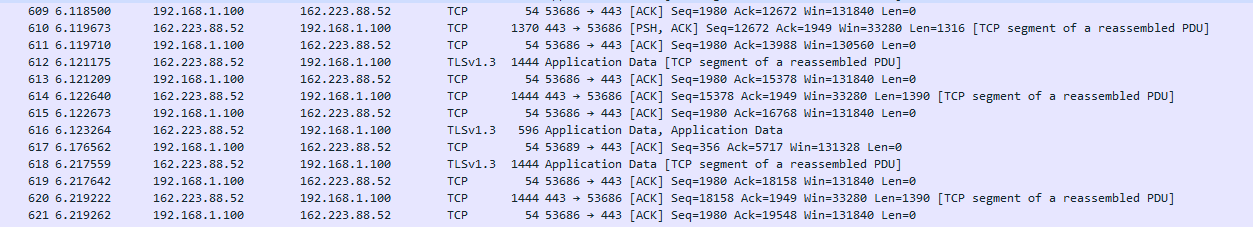
\includegraphics[width = 0.5 \textwidth]{images/5.png}
\end{center}

از آن‌جایی که این آی‌پی در آمریکا قرار دارد و درخواست‌های ما از طریق آن به \lr{Oracle} منتقل می‌شود، \lr{Oracle} تحریم را اعمال نکرده و اطلاعات را به سرورهای شکن فرستاده و از آن طریق پاسخ مربوطه به ما بر می‌گردد.

در مورد مواردی که تحریم نیستند، آدرس ای‌پی تغییری نمی‌کند و در این زمینه شکن تغییری در روند کار ایجاد نکرده و مانند یک \lr{DNS-Server} معمولی عمل می‌کند.


نتایجی که برای فیسبوک بر می‌گردد به صورت زیر است:

		\begin{center}
	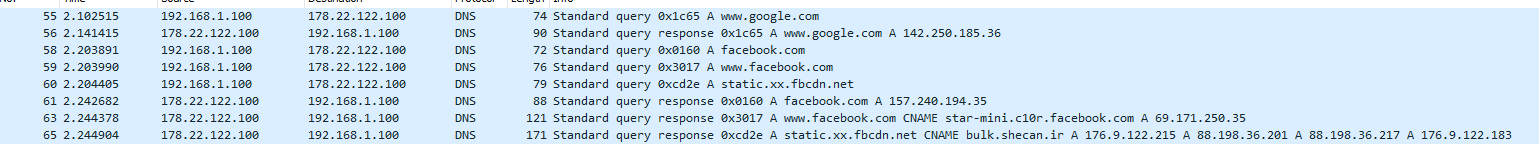
\includegraphics[width = 0.5 \textwidth]{images/6.png}
\end{center}

آی‌پی‌هایی که با آدرس‌های
\lr{\Verb+69.171.250.35+}
و
\lr{\Verb+157.240.194.35+}
برگردانده می‌شوند، هر دو واقعا متعلق به فیسبوک هستند. اما با این حال اگر پکت‌های TCP جا به جا شده به این IP را مشاهده کنیم وضعیت زیر را می‌بینیم:

		\begin{center}
	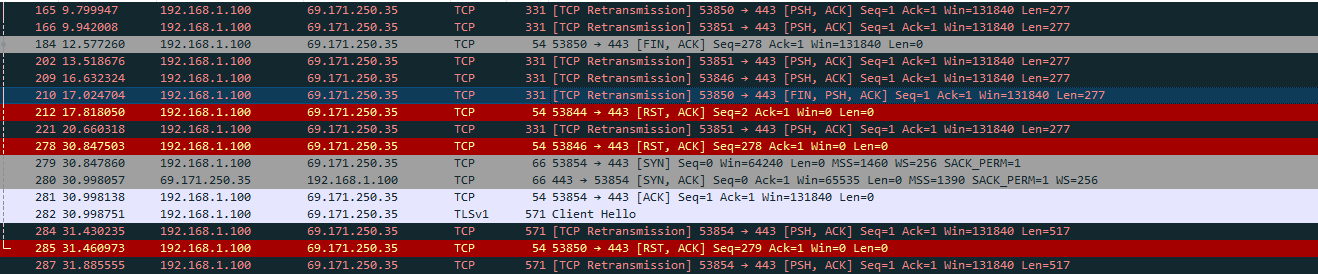
\includegraphics[width = 0.5 \textwidth]{images/7.png}
	\end{center}

مشاهده می‌شود که اکثر موارد به رنگ سیاه یا قرمز هستند. سیاه با حروف قرمز به معنی \lr{BAD TCP} و قرمز با حروف زرد به معنی \lr{TCP RST} است. تقریبا هیچ‌کدام از پکت‌های ارسالی ما به درستی به فیسبوک منتقل نشده‌اند. این بدین معنی است که فیلترینگ اعمال شده برای فیسبوک تنها در لایه \lr{DNS} نیست. بلکه فیلترینگ‌های دیگری هم اعمال شده است که پکت‌ها را بعد از رسیدن به \lr{ISP}‌های داخلی، با توجه به آدرس آن که مربوط به فیسبوک است و جزو سایت‌های فیلتر شده است، \lr{Drop} می‌کند تا به فیسبوک نرسند.

در این مورد \lr{Shecan} هم نقش خاصی ایفا نکرده و صرفا آدرس واقعی سایت \lr{\Verb+www.facebook.com+} را به ما برگردانده است و از آن‌جایی که جزو سایت‌های تحریمی هم نیست، آدرس سرورهای \lr{\Verb+us1.shecan.ir+} را به ما نداده است.


\item

خیر همان طور که در بالا توضیح داده شد، روش کار شکن بدین صورت است که لیستی از سایت‌های تحریم شده دارد و برای آن سایت‌ها، آی‌پی مربوط به سرورهای خود شکن را که در کشور دیگری مستقر هستند به ما بر می‌گرداند. بدین ترتیب، ریکوئست‌های ما به آن سایت از طریق سرورهای شکن که به نوعی نقش \lr{Man in the Middle} را ایفا کرده است به آن سایت منتقل شده و جواب‌ها از طریق این سرور شکن به ما می‌رسد.

در مورد سایت‌های فیلتر شده، شکن یا عملکردی مانند \lr{DNS} های \lr{ISP} ها داشته و \lr{IP} نامعتبری بر می‌گرداند و یا این که نهایتا \lr{IP} واقعی آن سایت را به ما می‌دهد. حتی با وجود این \lr{IP} واقعی هم امکان دسترسی به سایت ممکن نیست چون درخواست ما در راه به سرورهای \lr{ISP} ها می‌رسد و در آن جا با توجه به به این که مقصد آن جزو \lr{Blacklist} سایت‌های فیلتر شده است، اجازه انتقال به آن داده نمی‌شود و \lr{Drop} می‌شود. فیلترینگ سایتی نظیر فیسبوک صرفا در لایه DNS اعمال نشده، بلکه در لایه‌های دیگر هم اعمال شده است که اجازه انتقال بسته‌های درخواستی ما داده نشود تا حتی با داشتن آی‌پی سایت هم نتوان به آن دسترسی پیدا کرد.


\item

در قسمت قبلی هم یکی از IP های facebook نوشته شد. آی‌پی دیگری که با متصل بودن VPN فرانسه بدست آمد، \lr{\Verb+ 179.60.195.36+} بود که واقعا IP ثبت شده شرکت Facebook بوده و موقعیت جغرافیایی آن هم در بلژیک است که همسایه فرانسه است.  در صورت وصل بودن VPN، اطلاعات از طریق پروتکل ESP به سرورهای VPN ارسال شده و از طریق آن اطلاعات مربوط به فیسبوک دریافت می‌شود و سایت بدون مشکل باز می‌شود. با این حال در صورت قطع VPN و تلاش برای دسترسی به این آی‌پی وضعیت بسته‌ها مشابه زیر خواهد بود:



	\begin{center}
	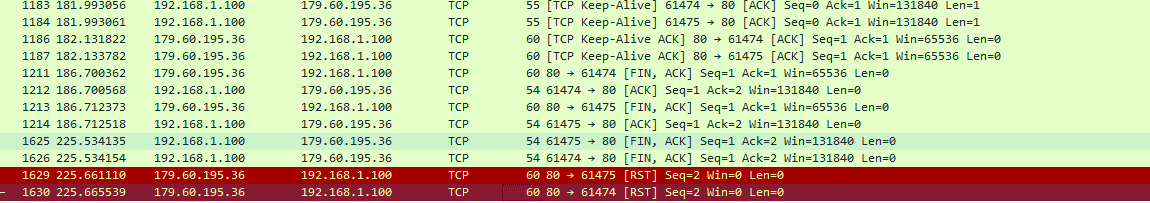
\includegraphics[width = 0.5 \textwidth]{images/8.png}
\end{center}

در ابتدا تعدادی بسته اولیه رد و بدل شده اما نتیجه نهایی به \lr{TCP RST} ختم شده است و همچنین با بررسی محتویات پیام‌های TCP آمده متوجه می‌شویم که همگی آن‌ها بسیار کوتاه هستند و اطلاعات کافی سایت را در بر ندارند.


\begin{center}
	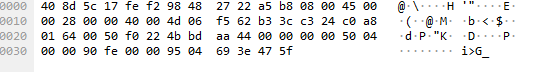
\includegraphics[width = 0.5 \textwidth]{images/9.png}
\end{center}

دلیل این موضوع هم این است که عملا فیلترینگ برای این سایت‌ها صرفا از لایه DNS نیست. بلکه به نوشته ویکی‌پدیا تکنولوژی \lr{Deep Packet Inspecting} در بخش فیلترینگ به کار رفته که جزئیات بسته‌های رد و بدل شده را بررسی می‌کند. بدین ترتیب مواردی نظیر آدرس مبدا یا مقصد و همچنین محتویات و کلمات استفاده شده در متن پیام در صورت رمزنگاری نشدن آن می‌تواند باعث بشود که Packet مورد نظر به عنوان محتوای فیلتر شده شناسایی شده و بعد از رسیدن به ISP ها Drop شود و در مواردی نظیر بالا تنها شامل رسیدن بسته‌هایی با متحوای بسیار کم هستیم.

علاوه بر این \textbf{نکته مهم} دیگری هم وجود دارد و آن هم بررسی بسته http ارسال شده است. با بررسی این بسته‌ها به مورد زیر می‌رسیم:

\begin{center}
	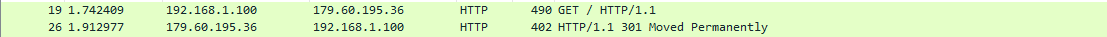
\includegraphics[width = 0.5 \textwidth]{images/10.png}
\end{center}

پاسخ دریافت شده برای درخواست \lr{\Verb+GET+} از این آدرس، کد \lr{\Verb+301 Moved Permanently+} است.


\begin{latin}
	\begin{verbatim}
	Hypertext Transfer Protocol
	HTTP/1.1 301 Moved Permanently\r\n
	Location: http://www.facebook.com/\r\n
	Content-Type: text/html; charset="utf-8"\r\n
	Date: Fri, 30 Apr 2021 15:11:44 GMT\r\n
	Alt-Svc: h3-29=":443"; ma=3600,h3-27=":443"; ma=3600\r\n
	Connection: keep-alive\r\n
	Content-Length: 0\r\n
	\r\n
	[HTTP response 1/1]
	[Time since request: 0.170568000 seconds]
	[Request in frame: 19]
	[Request URI: http://179.60.195.36/]
		
	\end{verbatim}
\end{latin}

آدرس جدید این سایت \lr{facebook.com} اعلام شده است. در نتیجه دوباره سیستم سعی‌ می‌کند از طریق DNS آدرس جدید را پیدا کند ولی در این زمینه هم با فیلترینگ مربوط به DNS رو به رو می‌شود و با آدرس \lr{\Verb+10.10.34.36+} رو‌به‌رو می‌شود که آدرس معتبری نیست.

	
\end{enumerate}

\section{سوال دوم}

\begin{enumerate}
	\item 
	پروتکل \lr{QUIC} یک پروتکل برای لایه انتقال است که توسط گوگل طراحی شده و  اکنون بعد از چندین سال طی مراحل آزمایشی، توسط \lr{IETF} به عنوان استاندارد جدید پذیرفته شده است. این پروتکل در مراحل اولیه توسط مروگر \lr{Chrome} و برای ارتباط با بعضی از سرویس‌ها و سایت‌های گوگل استفاده می‌شد اما اکنون شاهد گسترش استفاده آن و اضافه شدن پشتیبانی از آن به مرورگرهای دیگر هم اضافه شده است.
	
	هدف اصلی از طراحی \lr{QUIC}، ایجاد پروتکلی بوده است که هم به انتقال ترافیک \lr{HTTP} و \lr{HTTPS} سرعت بخشیده و هم امن‌تر باشد. این پروتکل بر پایه \lr{UDP} بنا شده است تا برای پیاده‌سازی آن نیاز به تغییر \lr{Middle-Box} های میانی ساختار شبکه نباشد. این پروتوکل سعی دارد با یکی کردن مراحل مربوط به \lr{Handshake} پروتکل‌های \lr{TCP} و همچنین پروتکل \lr{TLS} که برای \lr{HTTPS} استفاده می‌شود را در یک پروتکل یکپارچه کند و همچنین امکانات مربوط به \lr{Multiplexing} در \lr{HTTP/2} را هم به شکلی بهتر برای جلوگیری از \lr{HOL Blocking} پیاده‌سازی کند.
	
	\item
	
	در پروتکل \lr{HTTP/2} امکان \lr{Multiplexing} درخواست ها فراهم شد. به این شکل که به جای این که چندین \lr{Connection} از نوع \lr{TCP} برقرار شود که هر کدام اطلاعات بخشی از صفحه را دریافت کنند، یک اتصال \lr{TCP} ایجاد شده و بسته به این که هر قسمت متعلق به کدام بخش صفحه است، \lr{Multiplexing} صورت گرفته و به یکی از آن‌ها تعلق می‌گیرد.
	
	\begin{center}
		
		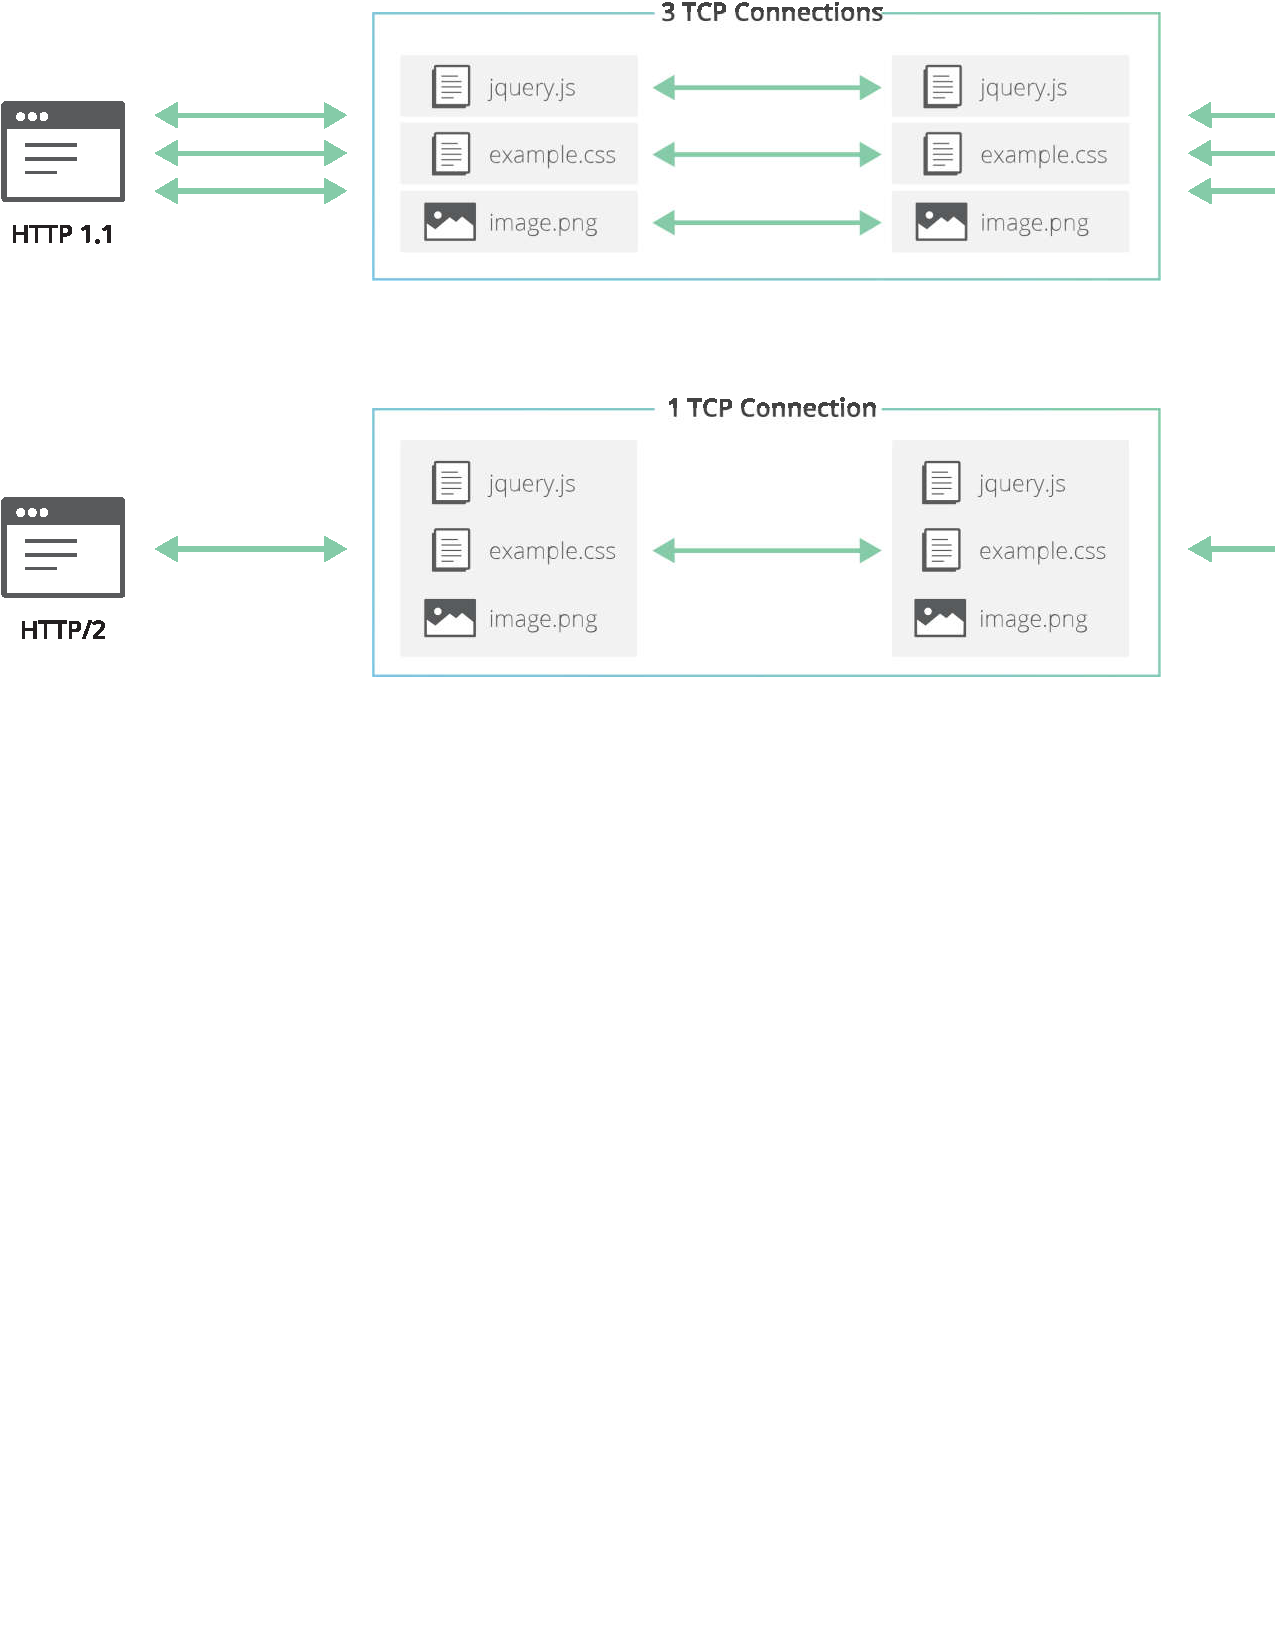
\includegraphics[width = 0.6\textwidth , trim=0 400 0 0]{images/multiplexing.pdf}
	\end{center}
	
	تنها ایرادی که در این زمینه وجود دارد مشکل \lr{Head of Line Blocking} است. در این حالت اگر یکی از پکت‌های \lr{TCP} از دست برود، باید منتظر ارسال مجدد آن بمانیم و عملا مزایای \lr{Multiplexing}‌ از بین می‌رود و با وجود تقسیم شدن به سگمنت‌های مختلف، همگی ‌آن‌ها معطل رسیدن بسته از دست رفته خواهند بود.
	
	با این حال \lr{QUIC} از پایه به این شکل طراحی شده است که \lr{Multiplexing} را به طور کامل پشتیبانی کند. این پروتکل قسمت‌های مختلف صفحه را به \lr{Stream} های مجزا تقسیم می‌:ند. از دست رفتن داده در یک پکت خاص مربوط به یک \lr{Stream} مشخص، تنها منجر به معطل شدن همان \lr{Stream} شده و بقیه \lr{Stream Frame} ها می‌توانند با موفقیت بعد از دریافت به بخش مربوطه متصل شده و معطل رسیدن بسته \lr{Stream} از دست رفته نخواهند بود. در این اتصال استریم‌های مختلف \lr{HTTP} می‌توانند به استریم‌های مختلف \lr{QUIC} مرتبط بشوند. ضمن این که همه این استریم‌ها از یک کانکشن \lr{QUIC} استفاده کرده و در نتیجه نیازی به انجام \lr{handshake}‌ های مجدد ندارند.


نتیجه نهایی همه این موارد این است که در اکثر اوقات، از دست رفتن یک پکت در یک استریم منجر به ایرادی یا بلاک شدن بقیه نمی‌شود و بقیه می‌توانند با موفقیت مراحل انتقال خود را انجام بدهند.


\item

اتصال \lr{QUIC} را کلاینت که یکی از \lr{Endpoint} های اتصال است برقرار می‌کند. در \lr{QUIC} اطلاعات مربوط به ورژن، رمزنگاری و \lr{Handshake} های اولیه همگی با هم صورت می‌گیرند تا تاخیری که در اثر مراحل شروع کار صورت می‌گیرد کاهش یابد. 

هر کدام از پکت‌های اولیه که توسط کلاینت ارسال می‌شوند باید فلگ مربوط به ورژن را به حالت \lr{On} در آورده و جزییات ورژن مورد استفاده را در میان بگذراند. تمامی پکت‌های ارسالی کلاینت در ابتدا این فلگ را در حالت \lr{On} می گذراند تا زمانی که یک جواب از سمت سرور با فلگ ورژن \lr{Off} دریافت شود. سرور هم پس از این که اولین پکتی از کلاینت را دریافت کرد که فلگ ورژن آن Off \lr{بود}، باید پکت‌های دیگری که با فلگ \lr{On} ممکن است به دلیل تاخیر دریافت شوند را نادیده بگیرد.

هنگامی که سرور یک پکت با \lr{Connection ID} جدیدی را دریافت می‌کند، ورژن آن را با ورژن‌هایی که پشتیبانی می‌کند مقایسه می‌:ند و اگر از آن پشتیبانی می‌کرد، تا انتهای عمر این اتصال از آن استفاده می‌کند.

در صورتی که این ورژن قابل قبول نباشد، با تاخیر یک \lr{Round-Trip Time} از سمت سرور یک پکت برای مذاکره در مورد ورژن به کلاینت ارسال می‌شود که در آن فلگ ورژن On بوده و لیست ورژن‌های قابل قبول در آن آمده است. کلاینت هم پس از دریافت این موضوع، یکی از آن آن پروتکل‌ّا را انتخاب کرده و براساس آن اطلاعات را از ابتدا باز ارسال می‌کند.

برای جلوگیری از حملات \lr{Donwgrading}، جزییات مربوط به ورژن که کلاینت در ابتدا مشخص کرده و ورژن‌های پشتیبانی شده توسط سرور در اطلاعات مربوط به \lr{Handshake} رمزنگاری هم قرار می‌گیرند تا کلاینت با چک کردن آن‌ها بتواند از صحت این اطلاعات اطمینان حاصل کند.

در همین مراحل اطلاعات مربوط به رمزنگاری و \lr{Handshake} اولیه لایه انتقال هم انجام می‌گیرد. یعنی همزمان مراحل انتقال جزییات رمزنگاری و \lr{Handshake} لازم با هم انجام می‌شود. \lr{QUIC} در ورژن‌های فعلی خود از پروتوکل \lr{TLS} برای رمزنگاری استفاده می‌کند اما این امکان وجود دارد که در آینده امکان استفاده از پروتکل‌های دیگری هم مهیا بشود. در حین انجام عملیات \lr{Handshake}، اطلاعات سطح \lr{Application} هم امکان انتقال دارند. به شکل ساده، ارتباط اولیه رمزنگاری به چنین شکلی قابل انجام است:

\begin{center}

\begin{latin}
	\begin{Verbatim}
	Client                                               Server
	
	Initial (CRYPTO)
	0-RTT (*)              ----------->
							Initial (CRYPTO)
							Handshake (CRYPTO)
				<----------                1-RTT (*)
	Handshake (CRYPTO)
	1-RTT (*)              ----------->
				<----------   1-RTT (HANDSHAKE_DONE)
	
	1-RTT                  <=========>                    1-RTT
	\end{Verbatim}
\end{latin}
	
\end{center}

	در همین مرحله، می‌توان اطلاعات مربوط به \lr{Explicit Congestion Notification} را هم منتقل کرد که مشخص کند آیا یکی از طرفین درگیر \lr{Congestion} شده است یا نه که طرف دیگر بداند باید با نرخ ارسال پایین اطلاعات را ارسال کند یا نه.
	
	
	در مورد اتمام اتصال، روش به این صورت است که اتصالات بعد از این که در وضعیت Idle‌ یا بلااستفاده قرار بگیرند، برای مدتی باز می‌ماند و پس از گذشت آن زمان، سرور اتصال را قطع می‌:ند. این قطع شدن اتصال لزوما با خبر کردن کلاینت همراه نخواهد بود چون اگر این اتصال در دستگاه‌های همراه (موبایل‌ها) برقرار شود، این کار نیازمندی فعال‌سازی دوباره اینترنت در این دستگاه‌ها بوده و منجر به مصرف برق می شود. در اصل به طور کلی دو نوع بسته شدن اتصال وجود دارد:
	
\begin{itemize}
	\item 
	خاموشی صریح: در این حالت یکی از \lr{Endpoint} ها یک فریم \lr{\Verb+CONNECTION\_CLOSE+} برای \lr{Endpoint}‌ دیگر ارسال می‌کند که آغازگر اتمام ارتباط است. \lr{Endpoint}‌دیگر می‌تواند یک فریم \lr{\Verb+GOAWAY+}‌ارسال کند که به معنی این است که به زودی ارتباط بسته خواهد شد. ارسال این سیگنال مشخص می‌کند که استریم‌های فعلی همچنان به کار خود اادامه می‌دهند تا به اتمام برسند ولی دیگر \lr{Stream} جدیدی ایجاد نخواهد شد تا بعد از اتمام کار قبلی‌ها، کار به اتمام برسد. بعد از اتمام کار دوباره \lr{\Verb+CONNECTION\_CLOSE+} ارسال می‌شود و اتصال به اتمام می‌رسد. اگر در حالی که هنوز استریم‌های ناتمام داریم این فریم ارسال شود، سمت دیگر باید این طور فرض کند که استریم‌ها به پایان نرسیده بودند ولی به شکل غیر منتظره بسته شدند.
	
	\item
	خاموشی ضمنی: تایم‌اوت پیش‌فرض برای قرار گرفتن یک اتصال در وضعیت بلااستفاده $30$ ثانیه است و در همان ابتدای ایجاد به عنوان یک پارامتر ضروری که \lr{\Verb+ICSL+} نام دارد باید مشخص بشود. حداکثر زمانی هم که می‌توان برای این کار تعیین کرد $10$ دقیقه است. اگر هیچ فعالیتی روی این اتصال به اندازه زمان مشخص شده وجود نداشته باشد، اتصال بسته می‌شود. در هنگام بسته شدن، به طور پیش‌فرض یک فریم \lr{\Verb+CONNECTION\_CLOSE+} ارسال می‌شود ولی می‌توان ارسال آن را غیرفعال کرد تا در شبکه‌هایی که هزینه ارسال بالاست (نظیر شبکه‌های موبایل)، بدون دریافت پیام جدید در سمت دیگر، اتصال بسته بشود.
	
	
\end{itemize}

در زیر دو مقایسه بین اتصال \lr{TCP} رایج به همراه رمزنگاری \lr{TLS} که برای شروع نیاز به دو \lr{RTT} دارد با پروتکل \lr{QUIC} که با یک \lr{RTT} این کار را انجام می‌دهد قرار گرفته است:


\begin{center}
	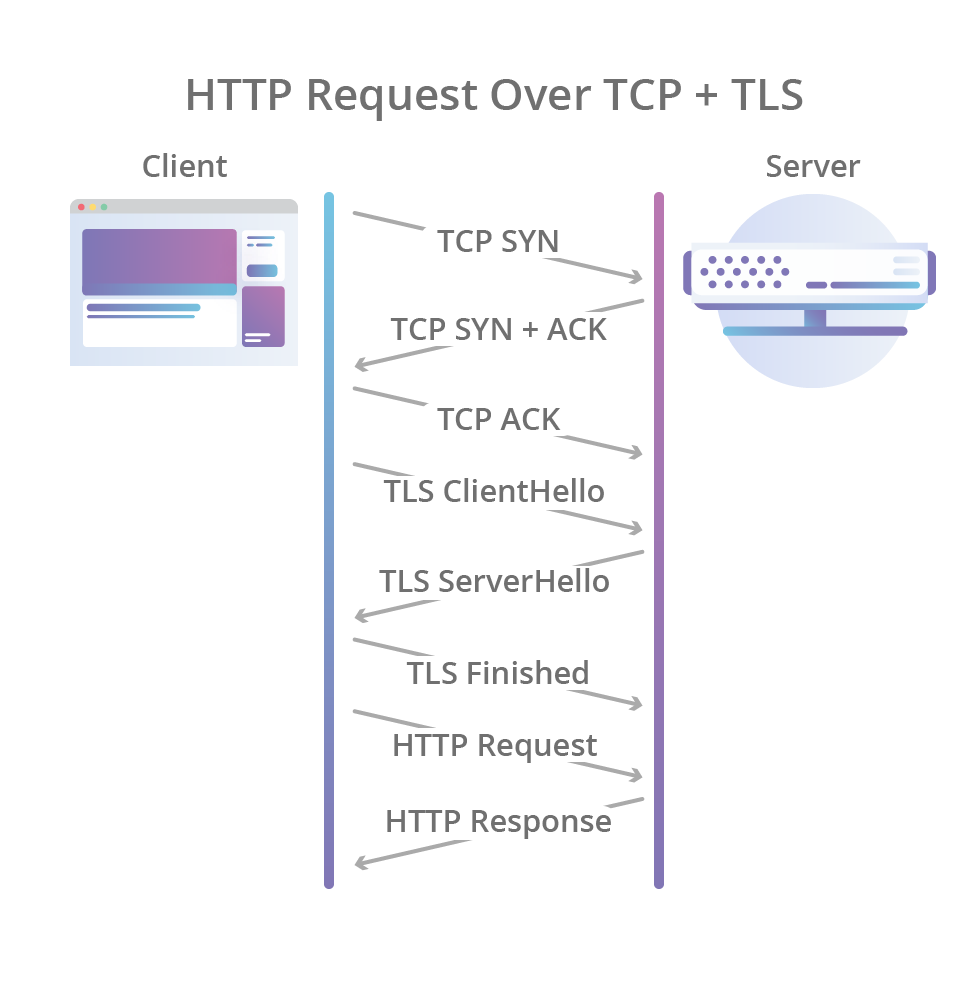
\includegraphics[width = 0.55 \textwidth]{images/11.png}
\end{center}


\begin{center}
	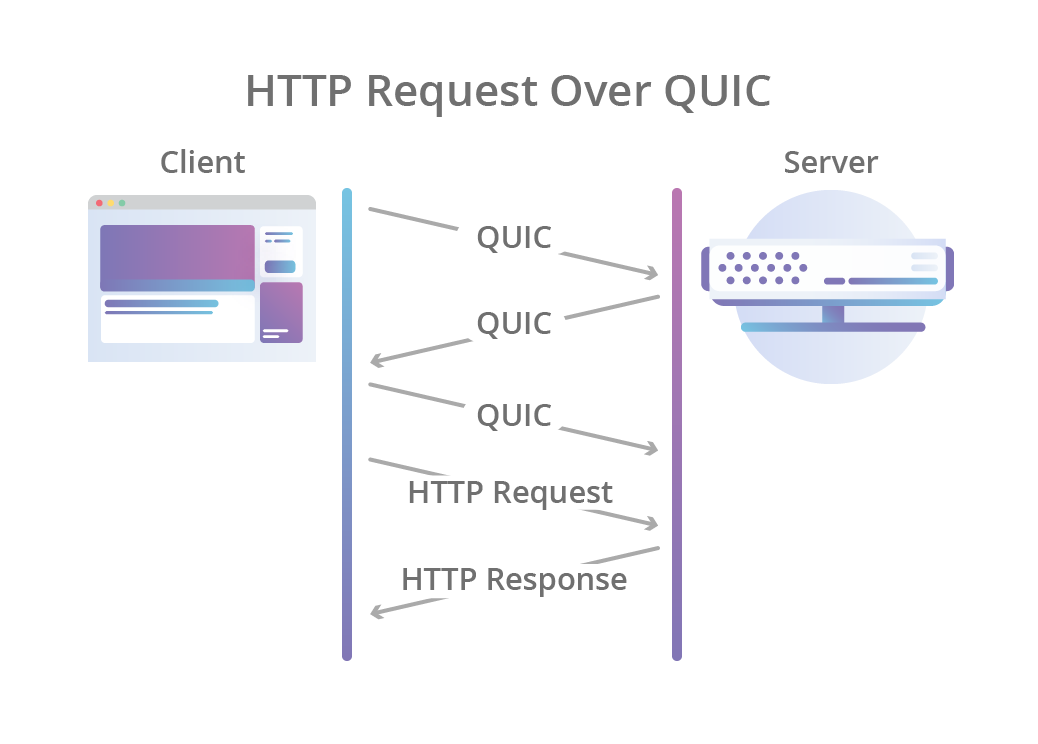
\includegraphics[width = 0.55 \textwidth]{images/12.png}
\end{center}


\item

این قسمت براساس درفت هشتم \lr{QUIC} نوشته شده است (لینک داده شده در صورت سوال درفت دوم \lr{QUIC} است):

\begin{latin}
\textcolor{Blue}{{\underline{\textcolor{Blue}{ \href{https://tools.ietf.org/html/draft-ietf-quic-transport-08}{https://tools.ietf.org/html/draft-ietf-quic-transport-08}}}}}
\end{latin}


	
	
\end{enumerate}



\end{document}



